\documentclass{article}

% Packages
\usepackage[danish]{babel}
\usepackage[utf8]{inputenc}
\usepackage[T1]{fontenc}
\usepackage{geometry}
\usepackage{listings}
\usepackage{amsfonts}
\usepackage{amsmath, amssymb, amsthm}
\usepackage{graphicx}
\graphicspath{{./}}

\begin{document}
\begin{titlepage}
    \vfill
    \clearpage\thispagestyle{empty}
    \centering
    {\Large \textbf{Mockup Project} }\vspace{0.5cm} \\
    {\textbf{Part 1} Database and Queries}
    \vfill
    {\textbf{Supervisor}}\\
    {Panagiotis Tampakis}
    \vfill
    {\textbf{Made by}}\\
    {Denis og Søren\\}
    \vskip6cm
\end{titlepage}

%%%%%%%%%%%
%%%%%%%%%%%
%%%%%%%%%%%
\section*{Abstract}
In this report we'll see how you can implement a database in PostgreSQL and
construct simple SQL queries to get the desired relation data.


%%%%%%%%%%%
%%%%%%%%%%%
%%%%%%%%%%%
\newpage
\section*{Preface}
This is a voluntarily project on the second semester of computer science in the course DM576 Database design.
The report is short and concise only documenting key decisions since we dedicated only a few hours to
the project as a whole.

\clearpage
\tableofcontents
%%%%%%%%%%%
%%%%%%%%%%%
%%%%%%%%%%%
\newpage
\input{Introduction.tex}


%%%%%%%%%%%
%%%%%%%%%%%
%%%%%%%%%%%
\newpage
\section{Database implementation}
\subsubsection{Integrity constraints}
\subsubsection{Record data}


%%%%%%%%%%%
%%%%%%%%%%%
%%%%%%%%%%%
\newpage
\section{Queries}

\subsubsection{}
\subsubsection{}


%%%%%%%%%%%
%%%%%%%%%%%
%%%%%%%%%%%
\newpage
\section{Appendix}
\subsection{Tables}
\begin{center}
    product: 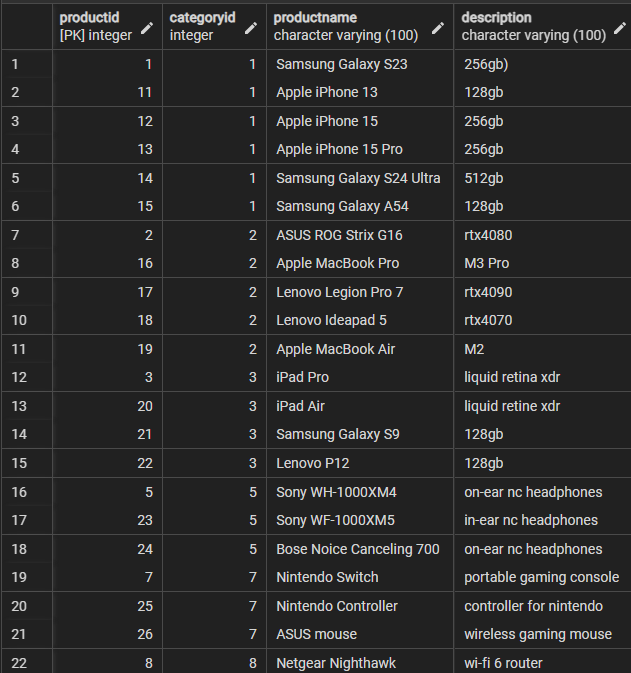
\includegraphics{{img/product_table}}
    \newpage
    product\_category: 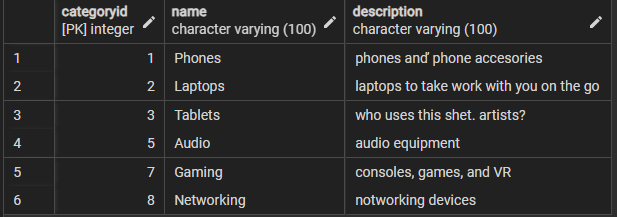
\includegraphics{{img/product_category_table}}
    supplier: 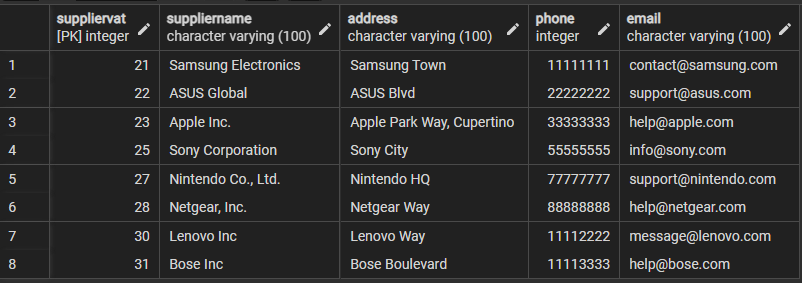
\includegraphics{{img/supplier_table}}
    supply: 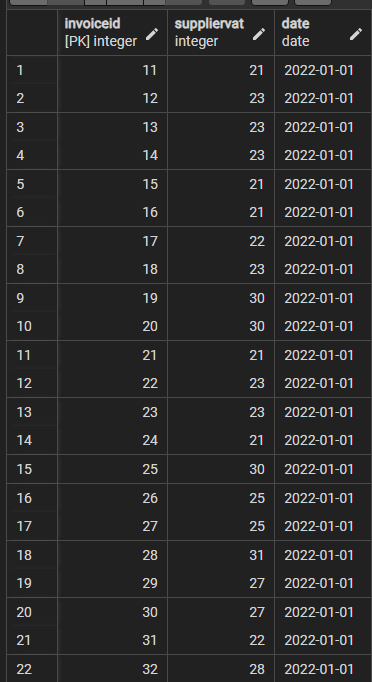
\includegraphics{{img/supply_table}}
    sale\_of\_product: 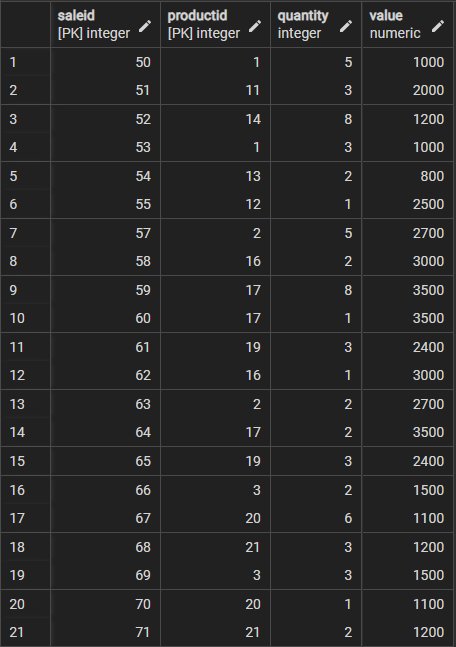
\includegraphics{{img/sale_of_product_table}}
    product\_return: 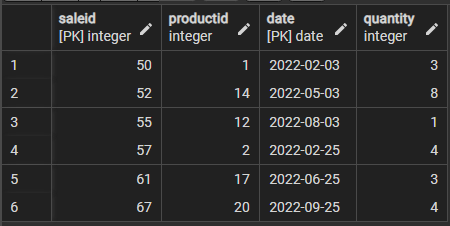
\includegraphics{{img/product_return_table}}
\end{center}
% \begin{lstlisting}[language=SQL, caption={constraints}, label={code:next}]
% \end{lstlisting}

% %%%%%%%%%%%
% %%%%%%%%%%%
% %%%%%%%%%%%
% \newpage
% \input{}
\end{document}
    








